\documentclass{article}
\usepackage[utf8]{inputenc}
\usepackage{graphicx} 
\title{Research Method: An Engineering Approach}
\author{Huynh Xuan Phung - Coursera}
\date{ }
\usepackage{color}   %May be necessary if you want to color links
\usepackage{hyperref}
\hypersetup{
    colorlinks=true, %set true if you want colored links
    linktoc=all,     %set to all if you want both sections and subsections linked
    linkcolor=blue,  %choose some color if you want links to stand out
} 
\begin{document}
 
\maketitle
 
\tableofcontents

\section{What does Knowledge Look Like?}

\subsection{Categories of knowledge}

\begin{figure}
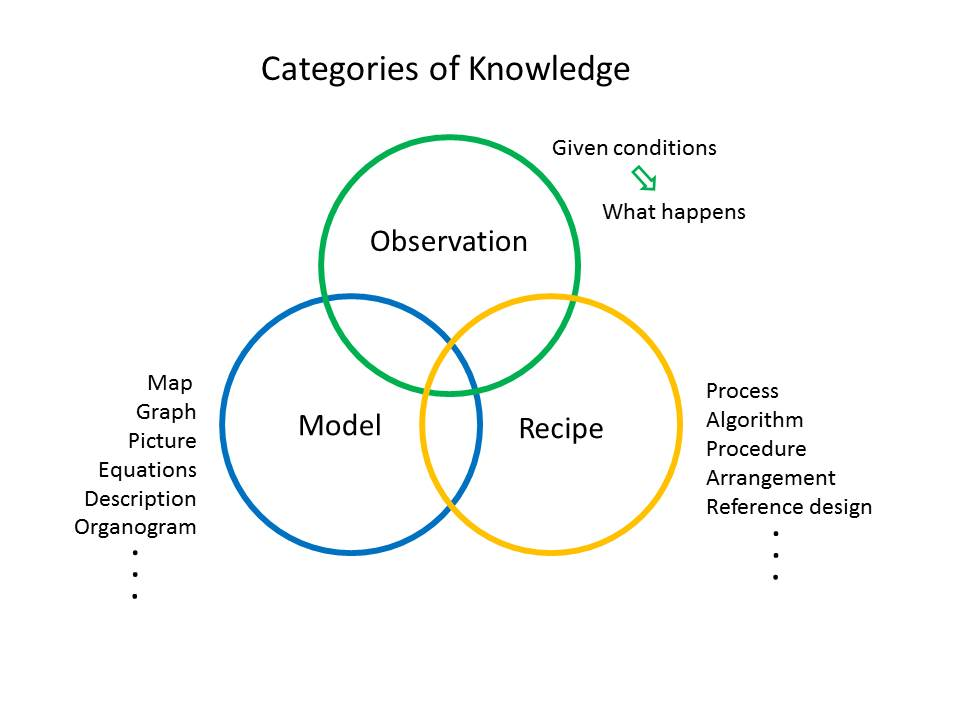
\includegraphics[scale=0.6]{figures/CategoriesOfKnowledge.png}
\caption{Categories of Knowledge.}
\end{figure}
 
An observation: I did some stuff and saw some stuff. 

Sometimes it could be that you use a different technique to carry out a complex calculation and you note that the time it takes to run the calculation is less. This is observational knowledge.

Models are a way of making sense of the world around us. They help us to be able to understand things. The model is probably the most common category of knowledge.

Models can take on many different forms such as:

\begin{itemize}
\item{Maps}
\item{Graphs}
\item{Pictures}
\item{Equations}
\item{Descriptions}
\item{Organograms}
\end{itemize}

Recipe is a way of arranging and doing things that brings about a desired effect.

Recipes can take on many different forms such as:
\begin{itemize}
\item{Processes}
\item{Algorithms}
\item{Procedures}
\item{Arrangements}
\item{Reference designs}
\end{itemize}

\subsection{Research Objective}
Research Objective is splitting into 3 parts:
\begin{itemize}
\item{Where the problem comes from}
\item{---Background and Context}
\item{What the problem is}
\item{---The problem and why it is important}
\item{What knowledge would we need}
\item{---The knowledge that is needed to deal with the problem}
\end{itemize} 

\subsection{Abstract forms}
It is possible to reduce research objectives down to such simple expression such as "How does A affect B?"

Questions
\begin{itemize}
\item{What method can be used to predict x?}
\item{Can x predict y?}
\item{Can process x improve process y?}
\end{itemize}



 
\end{document}